\documentclass[border=4pt]{standalone}
\usepackage{amsmath,amssymb}
\usepackage{tikz}
\usetikzlibrary{arrows.meta,positioning,calc}
\definecolor{cfg}{HTML}{2E7D46}\definecolor{mcfb}{HTML}{2166AC}\definecolor{negr}{HTML}{B03A2E}
\definecolor{inkc}{HTML}{1B1B1B}\definecolor{gy}{HTML}{6B7280}
\begin{document}
\hyphenpenalty=10000\exhyphenpenalty=10000
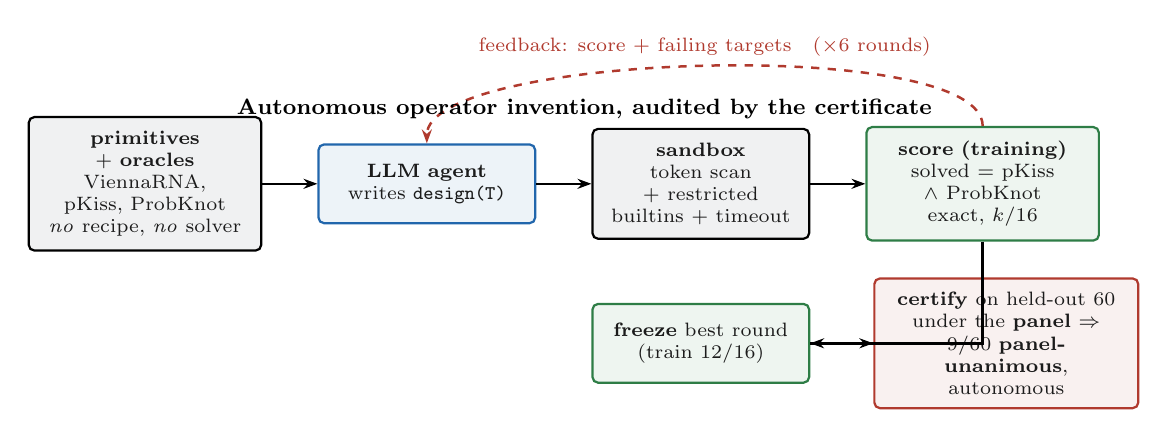
\begin{tikzpicture}[
  >={Stealth[length=5pt,width=3.6pt]},
  b/.style={draw, line width=0.8pt, rounded corners=2pt, align=center, inner sep=5pt, text=inkc, font=\scriptsize, minimum height=10mm},
  fl/.style={->, line width=0.9pt}, font=\scriptsize]

\node[b, fill=gy!10, text width=26mm] (prim) at (0,0)
  {\textbf{primitives $+$ oracles}\\ ViennaRNA, pKiss, ProbKnot\\ \emph{no} recipe, \emph{no} solver};
\node[b, draw=mcfb, fill=mcfb!8, text width=24mm, right=7mm of prim] (agent)
  {\textbf{LLM agent}\\ writes \texttt{design(T)}};
\node[b, fill=gy!10, text width=24mm, right=7mm of agent] (sand)
  {\textbf{sandbox}\\ token scan $+$ restricted\\ builtins $+$ timeout};
\node[b, draw=cfg, fill=cfg!8, text width=26mm, right=7mm of sand] (score)
  {\textbf{score (training)}\\ solved $=$ pKiss $\wedge$ ProbKnot\\ exact, $k/16$};

\draw[fl] (prim) -- (agent);
\draw[fl] (agent) -- (sand);
\draw[fl] (sand) -- (score);
% feedback (revise) loop: score -> agent, over the top
\draw[fl, draw=negr, dashed] (score.north) .. controls +(0,1.15) and +(0,1.15) .. node[above, font=\scriptsize, text=negr]{feedback: score $+$ failing targets \; ($\times 6$ rounds)} (agent.north);

% freeze + certify below
\node[b, draw=cfg, fill=cfg!8, text width=24mm, below=8mm of sand] (freeze)
  {\textbf{freeze} best round\\ (train $12/16$)};
\node[b, draw=negr, fill=negr!7, text width=30mm, right=8mm of freeze] (cert)
  {\textbf{certify} on held-out $60$\\ under the \textbf{panel} $\Rightarrow$\\ \textbf{$9/60$ panel-unanimous}, autonomous};
\draw[fl] (score.south) |- (freeze.east);
\draw[fl] (freeze) -- (cert);

\node[font=\footnotesize\bfseries, above=1.9mm of agent, xshift=20mm] {Autonomous operator invention, audited by the certificate};
\end{tikzpicture}
\end{document}
